% USE PDFLatex!
% to correctly render Swedish characters

\documentclass{popsci}

\usepackage[utf8]{inputenc}
\usepackage[swedish, english]{babel}

\usepackage{fancyhdr}
\usepackage{titling}
\usepackage{color}
\usepackage{colortbl}
\usepackage{graphicx}
\usepackage{flushend}
\usepackage{lmodern}


% Please specify the presentation date
\presentationsdag{2016-04-28}

% use either of these commands to specify the title of your thesis
% \examensarbete{}
% To create a title in two rows, leave examensarbete blank and fill in examensarbeteTwoRows.
\examensarbeteTwoRows{Application Specific Instruction-set Processor Using a Parametrizable multi-SIMD}{Synthesizeable Model Supporting Design Space Exploration}
\student{Magnus Hultin}
%\students{Magnus Hultin}{Mr X}
\supervisor{Flavius Gruian (LTH)}
\examiner{Krzysztof Kuchcinski (LTH)}

% Your pop-sci title should be different (more catchy) than your thesis title
\title{Parametrisk processor modell för design utforskning}


\begin{document}

% not more than 4 rows!
\theabstract{Applikations-specifika processorer är allt mer vanligt för få ut rätt prestanda med så lite resurser som möjligt. Detta arbete har en parametrisk modell för att kunna testa hur mycket resurser som behövs för en specifik applikation.}


{\noindent För att öka prestandan i dagens processorer finns det vektorenheter och flera kärnor i processorer. Vektorenheten finns till för att kunna utföra en operation på en mängd data samtidigt och flera kärnor gör att man kan utföra fler instruktioner samtidigt. Ofta är processorerna designade för att kunna stödja en mängd olika datorprogram. Detta resulterar i att det blir kompromisser som kan påverka prestandan för vissa program och vara överflödigt för andra. I t.ex. videokameror, mobiltelefoner, medicinsk utrustning, digital kameror och annan inbyggd elektronik, kan man istället använda en processor som saknar vissa funktioner men som istället är mer energieffektiv. Man kan jämföra det med att frakta ett paket med en stor lastbil istället för att använda en mindre bil där samma paketet också skulle få plats.

I mitt examensarbete har jag skrivit en modell som kan användas för att snabbt designa en processor enligt vissa parametrar. Dessa parametrar väljs utifrån vilket eller vilka program man tänkta köra på den. Vissa program kan t.ex. lättare använda flera kärnor och vissa program kan använda korta eller längre vektorenheter för dess data.

%För att kunna välja vilken typ av processor som är rätt för den specifika applikationen krävs det ofta att man snabbt kan testa olika prototyper. Att implementera dessa till hårdvara kan ofta vara tidskrävande och ifall det visar sig att implementationen inte klarar dem kraven man ställt för prestanda och energieffektivitet, måste man designa för nya parametrar och mer tid har blivit slösat. %Om den här processen istället kan göras automatiskt utifrån dessa design-parametrar kan man teoretiskt spara en massa tid.
Modellen testades med olika multimedia program. Den mest beräkningsintensiva och mest upprepande delen av programmen användes. Dessa kallas för kärnor av programmen. Kärnorna som användes var ifrån MPEG och JPEG, som används för bildkomprimering och videokomprimering.

\begin{figure}[!bth] % Use pictures in your pop-vet!
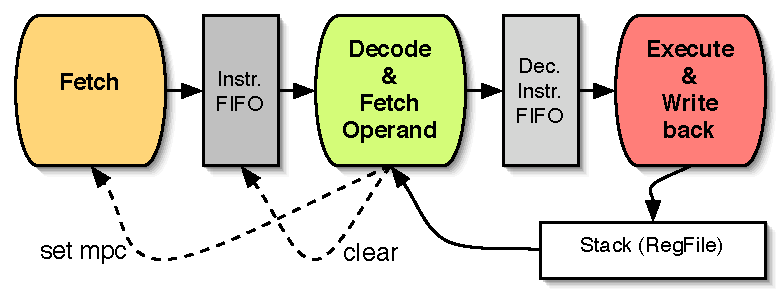
\includegraphics[width=\columnwidth]{samplePic.pdf} 
%\caption{En fin bild}
\end{figure}
Resultatet visar att det finns en prestanda vinst jämfört med generella processorer men att detta också ökar resurserna som behövs. Detta trots att den generella processorn har nästan dubbelt så hög klockfrekvens än dem applikations-specifika processorerna. Resultatet visar också att schemaläggning av instruktionerna i programmen spelar en stor roll för att kunna utnyttja resurserna som finns tillgängliga och därmed öka prestandan. Med den schemaläggningen som utnyttjade resurserna bäst var prestandan minst 79\% bättre än den generella processorn.
}

\end{document}
